\section{Natural Gas}
\label{sec:natural_gas}
%\addcontentsline{toc}{section}{\nameref{sec:natural_gas}}

\subsection{General}
As previously noted, only buildings that indicated natural gas being used \lstinline{NGUSED} were included in the samples for this major fuel use.  Then, one of each pair of predictors with correlations above 0.75 were removed, to avoid model selection issues. Numeric predictors were transformed via BoxCox methodology as well as centered and scaled.  Note, no further commentary will be made in the following sections unless it differs from previous sections.

\subsection{Response Analysis}

After filtering for this model's end-use, there are 6662 samples in the data set.  The same transformations were applied to this response variable as electricity. \textit{\hyperref[appendix:natural_gas:response]{Appendix}}

\subsection{Variable Selection - PCA}
RMSE: NA, Rsquared: NA\\
Top 5: \lstinline{EDSEATPerSf}, \lstinline{PBA.14[EDUCATION]}, \lstinline{STRLZR.1[YES]}, \lstinline{MCHEQP[NA]}, \lstinline{ACT2PCT}  \textit{\hyperref[appendix:natural_gas:pca]{Appendix}}

\subsection{Variable Selection - PLS}
RMSE: 73076, Rsquared: 0.293\\
Top 5: \lstinline{FDSEATPerSf}, \lstinline{HEATP}, \lstinline{RFGWINPerSf}, \lstinline{NWKERPerSf}, \lstinline{RGSTRNPerSf}\\
\\[0.1in]
The Rsquared and RMSE values are still on the poorer side compared to those in the electricity study, which suggests there is either a more complex relationship, or there is greater variance in response, given the available data. However, the presence of attribute which indicates the percent of the building that is heated (\lstinline{HEATP}) is promising.   \textit{\hyperref[appendix:natural_gas:pls]{Appendix}}

\subsection{Variable Selection - Random Forest}
RMSE: 175808, Rsquared: 0.193\\
Top 5: \lstinline{DRYCL.1[YES]}, \lstinline{FDSEATPerSf}, \lstinline{RFGWINPerSf}, \lstinline{LAUNDR.3[OFF-SITE]}, \lstinline{STRLSZR.1[YES]} 
\\[0.1in]
Again, the error values are much lower; however, the presesence of notable fuel-using equipment have been indicated to be of high importance. \textit{\hyperref[appendix:natural_gas:rf]{Appendix}}

\subsection{Variable Selection - Lasso}
RMSE: NA, Rsquared: NA\\

\subsection{Variable Selection - Forward Selection}
RMSE: 100385, Rsquared: 0.246\\
Top 5: \lstinline{FDSEATPerSf}, \lstinline{TVVIDEONPerSf}, \lstinline{NGWATR.2[NO]}, \lstinline{RGSTRNPerSf}, \lstinline{RFGWINPerSf}  \textit{\hyperref[appendix:natural_gas:lp]{Appendix}}

\subsection{Variable Selection - Recursive Feature Elimination}
RMSE: 59212, Rsquared: 0.523\\
Top 5: \lstinline{NWKERPerSf}, \lstinline{RFGICNPerSf}, \lstinline{RFGWINPerSf}, \lstinline{FDSEATPerSf}, \lstinline{RGSTRNPerSf}  \textit{\hyperref[appendix:natural_gas:rfe]{Appendix}}

\subsection{Variable Selection - Simple Neural Network}
RMSE: 69784, Rsquared: 0.334\\
Top 5: \lstinline{FDSEATPerSf}, \lstinline{RGSTRNPerSf}, \lstinline{DRYCL.1[YES]}, \lstinline{PBAPLUS.33[RESTAURANT/CAFETERIA]}, \lstinline{PBAPLUS.32[FAST FOOD]}  
\textit{\hyperref[appendix:natural_gas:snn]{Appendix}}

\subsection{Variable Selection - Selected Variable Analysis}
\begin{figure}[h]
\centering
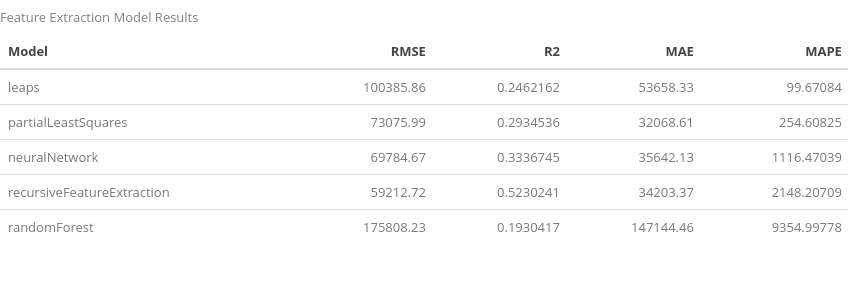
\includegraphics[width=.8\textwidth, height=0.25\textheight]{Images/natural_gas_psf_fe_summary.png}
\end{figure}
\begin{figure}[h]
\centering
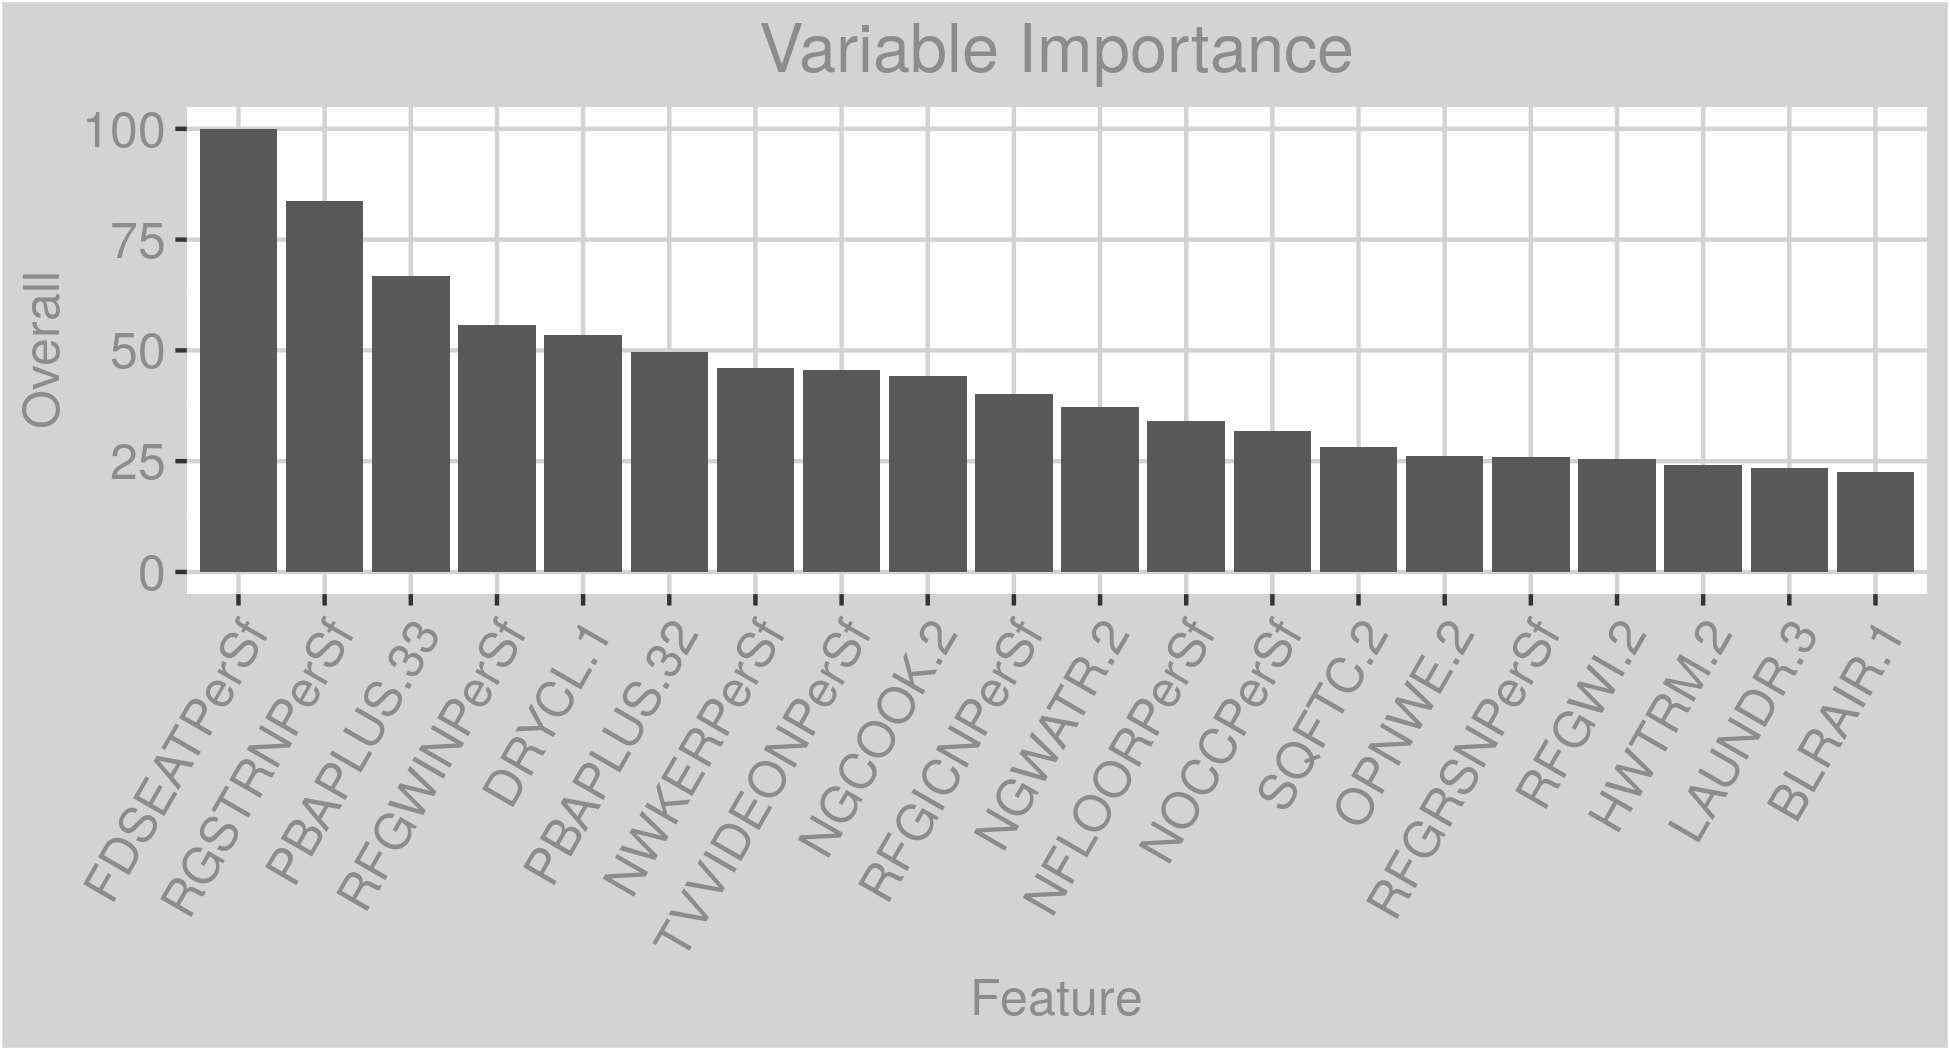
\includegraphics[width=.99\textwidth, height=0.375\textheight]{Images/natural_gas_psf_all_vars.png}
\end{figure}
\FloatBarrier

As with the electricity model, attributes related to occupancy seem to have made a large impact, possibly due to the need to heat ventilation air, especially given some of these occupancy types are associated with 24/7 operation.  Also as expected, cooking and large heating equipment attributes are high on the list.  Surprisingly, the number of floors per gross floor area has shown some importance, perhaps due to building shape and its relationship with heating needs (i.e. volume to area ratio). \textit{\hyperref[appendix:natural_gas:sva]{Appendix}}